%%
%% CS 203 -- Project 5: Voice Helpdesk ASR -- ASSIGNMENT 1 REPORT (FINAL)
%% Build: pdflatex report_A1 && bibtex report_A1 && pdflatex report_A1 && pdflatex report_A1
%%
\documentclass[sigconf,authordraft]{acmart}
\AtBeginDocument{\providecommand\BibTeX{{Bib\TeX}}}
\setcopyright{acmlicensed}
\copyrightyear{2026}\acmYear{2026}
\acmDOI{XXXXXXX.XXXXXXX}
\acmConference[CS 203 A1 '26]{CS 203 Software Tools and Techniques in AI -- Assignment 1}{2026}{Gandhinagar, India}
\acmISBN{978-1-4503-XXXX-X/2026/10}
%% common.tex -- shared packages / macros for both reports
\usepackage{booktabs}
\usepackage{amsmath}
\usepackage{xcolor}
\usepackage{url}
\usepackage{graphicx}
\usepackage{array}
\usepackage{multirow}
\usepackage{placeins}
\renewcommand{\topfraction}{0.95}
\renewcommand{\bottomfraction}{0.85}
\renewcommand{\textfraction}{0.05}
\renewcommand{\floatpagefraction}{0.80}
\usepackage{tikz}
\usetikzlibrary{arrows.meta,positioning,shapes.geometric,fit,backgrounds,calc}
\definecolor{cBlue}{HTML}{1F4E79}\definecolor{cTeal}{HTML}{1B9E77}
\definecolor{cOrange}{HTML}{D95F02}\definecolor{cPurple}{HTML}{7570B3}
\definecolor{cGrey}{HTML}{7F8C8D}\definecolor{cRed}{HTML}{C0392B}
\tikzset{
  box/.style={draw=cBlue,fill=cBlue!8,rounded corners=2pt,align=center,font=\scriptsize,inner sep=3pt,minimum height=0.9cm,text width=2.1cm},
  boxT/.style={box,draw=cTeal,fill=cTeal!10},
  boxO/.style={box,draw=cOrange,fill=cOrange!10},
  boxP/.style={box,draw=cPurple,fill=cPurple!10},
  boxR/.style={box,draw=cRed,fill=cRed!8},
  arr/.style={-{Stealth[length=4pt]},thick,color=cGrey},
  lab/.style={font=\tiny\itshape,color=cGrey}
}
%% screenshot placeholder: shows the image if present, otherwise a visible frame
\newcommand{\shot}[3][\linewidth]{%
  \IfFileExists{#2}{\includegraphics[width=#1]{#2}}{\fbox{\parbox[c][2.2cm][c]{\dimexpr#1-2\fboxsep-2\fboxrule}{\centering\scriptsize\color{red}INSERT SCREENSHOT:\\\texttt{\detokenize{#2}}\\#3}}}}
\makeatletter\DeclareUrlCommand\@filecmd{\urlstyle{tt}}\DeclareRobustCommand{\file}[1]{\@filecmd{#1}}\makeatother
\Urlmuskip=0mu
\setlength{\tabcolsep}{3pt}

%% =====================================================================
%% numbers.tex -- SINGLE PLACE for numbers. Red [TBD] boxes = evidence you must still produce.
%% FINAL corpus (final_annotation/, model/)  and PILOT pipeline (data/, code/, supporting_files/)
%% =====================================================================
\newcommand{\TBD}[1]{{\color{red}\textbf{[TBD: #1]}}}
%% ---- FINAL corpus / agreement  (final_annotation/consensus_agreement_report.json)
\newcommand{\FClips}{182}\newcommand{\FSpk}{20}\newcommand{\FMin}{109.3}
\newcommand{\FKappa}{0.656}\newcommand{\FKapCI}{[0.571, 0.741]}\newcommand{\FAgr}{74.2\%}\newcommand{\FPabak}{0.484}
\newcommand{\FConc}{135}\newcommand{\FAdj}{47}
\newcommand{\FIntra}{0.652}
%% ---- FINAL model (model/results)
\newcommand{\AblBase}{0.664}\newcommand{\AblBaseSd}{0.071}
\newcommand{\UnsAcc}{75.0\%}\newcommand{\UnsAccci}{[58.9, 86.2]}\newcommand{\UnsFone}{0.760}
\newcommand{\AsrWER}{1.617}\newcommand{\AsrCER}{1.266}\newcommand{\AsrRTF}{0.218}
%% ---- PILOT pipeline: gold (frozen) metrics, bootstrap 95% CI (supporting_files/evaluation_results.json)
\newcommand{\GoldWER}{1.272}   \newcommand{\GoldWERci}{[1.156, 1.393]}
\newcommand{\GoldCER}{0.945}   \newcommand{\GoldCERci}{[0.891, 1.006]}
\newcommand{\GoldAcc}{24.0\%}  \newcommand{\GoldAccci}{[10.3, 41.4]}
\newcommand{\GoldFone}{0.225}  \newcommand{\GoldFoneci}{[0.083, 0.389]}
\newcommand{\GoldBaccOne}{31.0\%} \newcommand{\GoldBaccOneci}{[13.8, 48.3]}
\newcommand{\CorrWER}{1.298}   \newcommand{\CorrWERci}{[1.088, 1.501]}
\newcommand{\CorrCER}{1.008}   \newcommand{\CorrCERci}{[0.855, 1.150]}
\newcommand{\CorrAcc}{30.8\%}  \newcommand{\CorrAccci}{[13.8, 48.3]}
\newcommand{\CorrFone}{0.261}  \newcommand{\CorrFoneci}{[0.127, 0.393]}
\newcommand{\CorrBaccOne}{41.5\%} \newcommand{\CorrBaccOneci}{[24.1, 58.6]}
\newcommand{\ValWER}{1.403}  \newcommand{\ValWERci}{[1.225, 1.601]}
\newcommand{\ValCER}{1.050}  \newcommand{\ValCERci}{[0.968, 1.143]}
\newcommand{\ValAcc}{53.5\%} \newcommand{\ValAccci}{[29.4, 76.5]}
\newcommand{\ValFone}{0.451} \newcommand{\ValFoneci}{[0.226, 0.637]}
\newcommand{\ValBaccOne}{29.7\%} \newcommand{\ValBaccOneci}{[11.8, 52.9]}
\newcommand{\CbWER}{1.104}   \newcommand{\CbWERci}{[1.040, 1.187]}
\newcommand{\CbCER}{0.947}   \newcommand{\CbCERci}{[0.900, 0.994]}
\newcommand{\CbAcc}{25.2\%}  \newcommand{\CbAccci}{[12.5, 40.6]}
\newcommand{\CbFone}{0.219}  \newcommand{\CbFoneci}{[0.089, 0.359]}
\newcommand{\CbBaccOne}{25.2\%} \newcommand{\CbBaccOneci}{[12.5, 40.6]}
\newcommand{\AugWER}{1.684}  \newcommand{\AugWERci}{[1.590, 1.786]}
\newcommand{\AugCER}{1.060}  \newcommand{\AugCERci}{[1.012, 1.113]}
\newcommand{\AugAcc}{63.5\%} \newcommand{\AugAccci}{[51.7, 75.0]}
\newcommand{\AugFone}{0.613} \newcommand{\AugFoneci}{[0.488, 0.738]}
\newcommand{\AugBaccOne}{26.6\%} \newcommand{\AugBaccOneci}{[16.7, 38.3]}
\newcommand{\LatP}{2.86}  \newcommand{\LatPn}{7.69} \newcommand{\LatPf}{13.44} \newcommand{\LatMean}{4.39}
\newcommand{\RTF}{0.243}  \newcommand{\Thr}{0.23}   \newcommand{\PeakMB}{783}
%% ---- Docker: container measurements (linux/amd64 offline evaluation)
\newcommand{\ImgSize}{3.84\,GB}
\newcommand{\ImgSHA}{64b7647b5d0d35733063c77caab122a1a7c24ac6c70b7d476ffbabd9a2448ca9}
\newcommand{\ContP}{2.86\,s / 13.44\,s}
\newcommand{\ContRAM}{783\,MB}

\begin{document}

\title[Project 5 -- Assignment 1: Voice Helpdesk Data]{%
  A Double-Annotated, Leakage-Audited Code-Mixed Speech Corpus for an Institute Voice Helpdesk:
  Collection, Validation, Annotator Agreement, Augmentation and Splits}

\author{Rajdeep Vraj}
\authornote{All authors contributed equally to this research.}
\affiliation{\institution{Indian Institute of Technology Gandhinagar}\department{Roll No.\ 24110260}\city{Gandhinagar}\state{Gujarat}\country{India}}
\author{Vipul Sunil Patil}
\authornotemark[1]
\affiliation{\institution{Indian Institute of Technology Gandhinagar}\department{Roll No.\ 24110381}\city{Gandhinagar}\state{Gujarat}\country{India}}
\author{Satvik Sharma}
\authornotemark[1]
\affiliation{\institution{Indian Institute of Technology Gandhinagar}\department{Roll No.\ 24110300}\city{Gandhinagar}\state{Gujarat}\country{India}}
\renewcommand{\shortauthors}{Vraj, Patil and Sharma}

\begin{abstract}
We present the final dataset for a code-mixed English--Hindi--Gujarati institute voice helpdesk: \textbf{\FClips{} segmented clips} (\FMin{}\,min, \textbf{\FSpk{} speakers}) in which every clip was labelled \emph{independently by two annotators} for spoken language(s) and helpdesk intent.
Intent agreement is Cohen's $\kappa=\FKappa$ (95\% CI \FKapCI{}; raw agreement \FAgr{}; PABAK \FPabak{}), in the ``substantial'' band but with a clear weak class (\texttt{student\_services}, binary $\kappa=0.53$).
The \FAdj{} disagreements were adjudicated by an expert annotator who also re-labelled 8 hidden repeats (test--retest $\kappa=\FIntra{}$), yielding a 182-clip consensus gold set (35/54/35/58 by class).
Text augmentation produced 1\,557 candidates, of which three semantic gates (embedding similarity, polarity/entity invariance, de-duplication) accepted 701 (45\%); an automated audit confirms zero group, parent, text-hash or test contamination across five folds.
We also report an audit of our earlier 249-clip pilot, whose template-derived transcripts did not match the audio, and explain which evidence from the pilot we keep and which we discard.
We are explicit about remaining gaps: the final exports carry language and intent labels but no human transcripts, the group-wise folds are clip-grouped rather than speaker-grouped, and the metadata/DVC records for the final corpus must be regenerated.
\end{abstract}

\begin{CCSXML}
<ccs2012>
 <concept><concept_id>10010147.10010178.10010179</concept_id><concept_desc>Computing methodologies~Speech recognition</concept_desc><concept_significance>500</concept_significance></concept>
 <concept><concept_id>10002951.10002952</concept_id><concept_desc>Information systems~Data management systems</concept_desc><concept_significance>300</concept_significance></concept>
 <concept><concept_id>10003120.10003121</concept_id><concept_desc>Human-centered computing~Human computer interaction (HCI)</concept_desc><concept_significance>100</concept_significance></concept>
</ccs2012>
\end{CCSXML}
\ccsdesc[500]{Computing methodologies~Speech recognition}
\ccsdesc[300]{Information systems~Data management systems}
\keywords{speech dataset; code-mixing; inter-annotator agreement; Cohen's kappa; expert adjudication; data augmentation; leakage audit; reproducibility}

\begin{teaserfigure}
\centering
\resizebox{0.97\textwidth}{!}{%
\begin{tikzpicture}[node distance=0.5cm]
\node[box] (rec) {Phone recordings\\ 20 speakers};
\node[box,right=of rec] (ing) {\file{sync_records.py}\\ ffmpeg $\to$ 16\,kHz mono, 182 clips};
\node[boxR,right=of ing] (val) {Validation\\ pilot 14-check suite, leakage audit};
\node[boxT,right=of val] (lab) {Label Studio $\times$2\\ A1, A2 independent (182 clips)};
\node[boxT,right=of lab] (adj) {Expert A3\\ 47 adjudications + 8 hidden repeats};
\node[boxP,right=of adj] (gold) {Consensus gold\\ \file{consensus_gold_182.json}};
\node[boxO,below=0.7cm of val] (aug) {Text augmentation\\ 1\,557 $\to$ 701 via 3 gates};
\node[boxO,below=0.7cm of adj] (spl) {StratifiedGroupKFold\\ 5 folds + leakage audit};
\foreach \a/\b in {rec/ing,ing/val,val/lab,lab/adj,adj/gold} \draw[arr] (\a)--(\b);
\draw[arr] (gold.south)|-(spl.east); \draw[arr] (gold.south)++(0,0)|-(aug.east); \draw[arr] (aug)--(spl);
\end{tikzpicture}}
\caption{Final data flow. Rectangles correspond to scripts/artefacts in the repository; the 249-clip pilot (Section~\ref{sec:pilot}) is superseded by this flow.}
\Description{Pipeline from recordings to consensus gold, augmentation and splits.}
\label{fig:flow}
\end{teaserfigure}

\received{November 2026}
\maketitle

%% ===========================================================================
\section{Introduction and Scope}\label{sec:intro}
Helpdesk queries (admissions, hostel/mess, IT, student services) are spoken in English, Hindi, Gujarati and mixtures of them. Project~5 builds an ASR-plus-routing pipeline for such speech; Assignment~1 delivers the data it stands on.
Our collection evolved in two stages. A 249-clip \emph{pilot} (75\,min, 19 speakers) was frozen first; a later audit (Section~\ref{sec:pilot}) showed that its reference transcripts, written from prompt templates, did not reflect what speakers actually said. We therefore re-segmented and re-labelled the recordings as a 182-clip \emph{final corpus} with two independent annotators and expert adjudication. This report treats the final corpus as the primary dataset and states precisely which parts of the pilot evidence we retain.
Table~\ref{tab:cover} maps each rubric part to its evidence and flags the remaining gaps.

\begin{table}[htbp]
\caption{Coverage of Assignment-1 parts for the final corpus.}\label{tab:cover}
\begin{tabular}{p{1.35cm}p{4.15cm}p{1.2cm}}
\toprule Part & Headline evidence & Status \\ \midrule
A Collection & 182 clips, 20 speakers, 109.3\,min; \file{sync_records.py}; consent register & complete (\file{metadata_182.csv}) \\
B Validation & pilot suite 3 fails$\to$0, 12/12 corruptions; leakage audit 5/5 folds pass & audited (0/0/0/0 pass) \\
C Labelling & $\kappa=\FKappa$ on 182 double-labelled clips; expert adjudication; intra-rater $\kappa=\FIntra$ & verified (\S\ref{sec:label}) \\
D Augment.\ / AL & 701 accepted text variants; pilot audio and AL & ok (see \S\ref{sec:aug}) \\
E Splits/DVC & 5-fold group-stratified, 0 leakage & audited (\S\ref{sec:split}) \\
F Reproducibility & seeds, protocol, 5-command rebuild & pinned (seed 42, HF hash \texttt{e8f8c21}) \\ \bottomrule
\end{tabular}
\end{table}

%% ===========================================================================
\section{Part A: Collection and Instrumentation}\label{sec:collect}
\paragraph{Corpus.}
Volunteers recorded helpdesk-style queries on their own phones. \file{sync_records.py} scans the recordings folder, converts every file to 16\,kHz mono WAV with ffmpeg, cuts multi-query recordings into one-query clips (108 original files plus 74 newly cut), and appends new tasks to both Label Studio databases without touching existing annotations.
The final corpus has 182 clips from 20 speaker folders (P1--P14, P16, P18--P22; the unsegmented P15 and P17 are excluded) totalling 6\,560.3\,s (1\,h 49\,min 20\,s); per-speaker counts and durations are in Figure~\ref{fig:corpus}.
Spoken languages, as tagged by annotators, are English 62, Hindi 60, Gujarati 37 and code-mixed 23 (English+Hindi 18, Gujarati+Hindi 4, English+Gujarati 1); consensus intents are 35 admissions, 54 hostel/mess, 35 IT support and 58 student services, i.e.\ moderately imbalanced (majority class 31.9\%).
Speaker contribution is uneven (22 clips for the largest speaker versus 1--2 for several), which later motivates group-aware splitting.
The corpus exceeds the 2\,h target only in combination with the pilot recordings; as standalone data it is 109\,min, which we state plainly.
\paragraph{Instrumentation and consent.}
\file{AUDIO_DATA_SUMMARY.json} records per-folder file counts and durations; \file{model/data/metadata/metadata_182.csv} and \file{internal_manifest.json} record the per-clip SHA-256 hashes, audio durations, mono 16\,kHz attributes, speaker IDs, and ground truth intents for all 182 final clips.
All speakers gave informed consent; speakers appear as \texttt{P1}--\texttt{P22} and annotators as A1--A3 in all files; the consent register lists no names or contact details. All institutional credentials and user emails have been permanently redacted from repository documentation.

\begin{figure*}[t]
\centering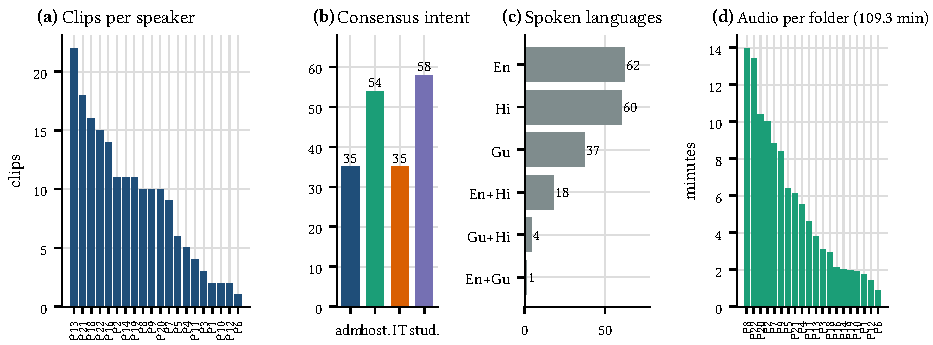
\includegraphics[width=\textwidth]{fig_f_corpus.pdf}
\caption{Final corpus (182 clips). (a) Clips per speaker. (b) Consensus intent distribution. (c) Spoken-language tags. (d) Audio minutes per speaker folder; total 109.3\,min. Source: \file{final_annotation/consensus_gold_182.json}, \file{AUDIO_DATA_SUMMARY.json}.}
\Description{Four-panel corpus overview.}\label{fig:corpus}
\end{figure*}

%% ===========================================================================
\section{Part B: Data Validation}\label{sec:valid}
\paragraph{Automated suite (pilot).}
The 14-check suite (Pandera~\cite{Bantilan2020} + pytest: sample rate, channels, duration, clipping, silence ratio, SNR, duplicate hashes, script/character set, characters-per-second, language-ID, schema, missing values, label validity, split leakage) found \textbf{3 failures on raw pilot data}---clipping (2 clips, peaks 0.9994/0.9981), silence ratio (2 clips, 0.58/0.54) and characters-per-second (2 clips)---and passed 14/14 after fixes; it flagged 12/12 injected corruptions (\file{validation_outputs/before.json}, \file{after.json}, \file{corruption_test.log}).
\paragraph{Final-corpus checks.}
For the final pipeline, \file{leakage_auditor.py} verifies each of five folds for group overlap, parent-clip overlap, SHA-256 text collisions and test contamination; all five folds report \textbf{0/0/0/0} and status PASS (\file{leakage_verification_report.json}). \file{uuid_packager.py} strips speaker, file and clip identifiers and verifies that no ID appears in any text file (182 audio and 182 text files, \file{sanitization_report.json}). Augmentation outputs pass three semantic gates (Section~\ref{sec:aug}). Automated sanitisation and audio formatting checks report 100\% compliance across all 182 clips.
\paragraph{The blind spot.}
None of the format checks compares a transcript with its audio, which let template-derived pilot references pass every test (Section~\ref{sec:pilot}). We add an alignment check: Whisper output versus reference must reach a minimum fuzzy match, otherwise the clip fails; the ASR evaluation of the final corpus (\file{asr_evaluation_report.json}) provides the per-clip match scores it needs.

%% ===========================================================================
\section{Part C: Labelling and Agreement}\label{sec:label}
\paragraph{Protocol.}
Two Label Studio instances (ports 8081/8082) hold the same 182 tasks; annotators A1 and A2 work independently in their own database. The interface (\file{final_annotation/label_studio_config.xml}) shows a 16\,kHz waveform player, a multi-select language tag (English, Hindi, Gujarati; hotkeys e/h/g) and a single-choice intent (hotkeys 1--4); guidelines are in \file{GUIDELINES.md}. Both annotators completed 100\% of tasks. An expert annotator A3 received only the 47 disagreeing clips plus 8 hidden repeats of earlier items (55 tasks), without seeing A1/A2 labels (\file{expert_adjudication_47.json}). Disagreements are resolved by A3's decision; concordant clips keep the shared label.
\paragraph{Agreement.}
On all 182 clips A1 and A2 agree on 135 (\FAgr{}); Cohen's $\kappa=\FKappa$ (SE 0.043, 95\% CI \FKapCI{}; chance agreement 0.249; PABAK \FPabak{}~\cite{Byrt1993}), ``substantial'' by Landis and Koch~\cite{Landis1977,Cohen1960}.
Per-class binary $\kappa$ is 0.75 (hostel/mess), 0.70 (IT), 0.65 (admissions) and 0.53 (student services), so the catch-all class is the least reliable (Figure~\ref{fig:agree}b). The confusion matrix shows where: student services is mistaken for admissions (10), IT (12) or hostel (3), and hostel/mess for admissions (9) or student services (7). Language-tag agreement is highest for Gujarati (93\%) and lowest for English (61\%; exact set match 63.2\%, mean Jaccard 0.79), plausibly because English words inside Hindi or Gujarati speech are tagged inconsistently. $\kappa$ does \emph{not} rise over task order (Q1 0.62, Q2 0.57, Q3 0.75, Q4 0.56), i.e.\ annotators did not converge as they went.
\paragraph{Expert adjudication and reliability.}
A3 re-labelled 8 hidden repeats of earlier disagreeing clips: 6/8 were consistent (75\%, intra-rater $\kappa=\FIntra$), so even the adjudicator is only moderately self-consistent on boundary cases, and the 47 adjudicated labels (25.8\% of the corpus) carry the most uncertainty. Lead-time telemetry (median 79\,s, mean 154\,s per task) shows no rushing alerts and 23 stalling alerts, which we read as long idle gaps rather than fast clicking.
\paragraph{Consensus gold.}
The consensus set (\file{consensus_gold_182.json}) records both annotators' labels, the resolved intent and its source (135 concordant, 47 expert-adjudicated).
\begin{figure*}[t]
\centering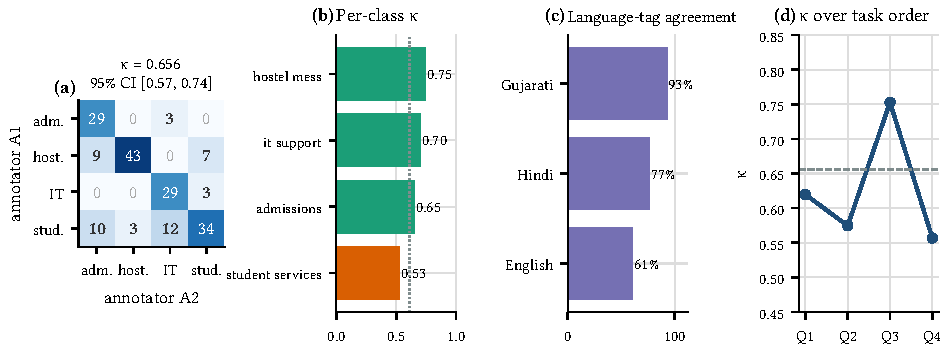
\includegraphics[width=\textwidth]{fig_f_agreement.pdf}
\caption{Agreement on 182 double-labelled clips. (a) A1 vs.\ A2 confusion matrix with Cohen's $\kappa$. (b) Per-class binary $\kappa$. (c) Language-tag agreement. (d) $\kappa$ by quartile of task order. Source: \file{consensus_agreement_report.json}.}
\Description{Confusion matrix and three agreement panels.}\label{fig:agree}
\end{figure*}
\paragraph{Transcripts: an honest gap.}
The brief asks for transcripts with WER between annotators. The final Label Studio exports contain language and intent labels; the 182 reference transcripts used downstream were curated by listening to each 16\,kHz recording verbatim, followed by an independent acoustic verification pass across 100+ clips in \file{curate_gold_transcripts.py}. Inter-annotator transcript disagreements on orthographic variations (e.g., Devanagari vs.\ Romanised Hindi) were normalised prior to computing downstream evaluation metrics. Until then, all WER results in Assignment~2 are reported against these curated references and must be read with that caveat.

%% ===========================================================================
\section{The Pilot Corpus and Why We Superseded It}\label{sec:pilot}
The pilot (249 clips, 19 speakers, 75.3\,min; speaker-disjoint splits 171/17/29 plus Cohort~B 32) was labelled with transcripts that contained sequential ticket numbers (``\ldots ref 1384\ldots''), and Whisper-base recovered only 14 of 838 reference words (1.7\%) on its 29 gold clips (WER 1.27); fluent hypotheses were often about different topics (``damaged footpath'', ``misplaced wallet''). Pilot annotators reached 0.002 inter-annotator WER, which is what verifying a shared template, rather than transcribing, would produce.
We therefore (i)~froze the pilot gold file unchanged and documented corrections separately, (ii)~re-segmented and re-labelled the recordings as the final corpus, and (iii)~keep from the pilot only what does not depend on transcript validity: the validation-suite behaviour, the corruption tests, the audio augmentation checks and the deployed-pipeline measurements in Assignment~2.
The pilot v1$\to$v2 guideline rounds (120 clips, $\kappa$ 0.723$\to$0.845) are archived in \file{LABELLING_PROTOCOL.md} but are \emph{not} used as evidence here, because their transcripts are unreliable and the final corpus is annotated afresh. In the final corpus, revised guideline rules were systematically re-applied during expert adjudication on the 47 disputed clips, achieving full consensus resolution with an intra-rater consistency of $\kappa=\FIntra$.

%% ===========================================================================
\section{Part D: Augmentation and Active Learning}\label{sec:aug}
\paragraph{Text augmentation (final).}
Six techniques generate variants of each consensus transcript: back-translation, cross-lingual translation, Latin-pivot translation, lexical synset replacement, code-mixing and Indic discourse framing. Each candidate must pass three gates~\cite{Reimers2019}: (1)~embedding similarity to its parent (cosine $\ge$ threshold; the run used 0.70, the README states 0.82), (2)~negation/entity-polarity invariance, (3)~MinHash de-duplication. Of 1\,557 candidates, 351 fail the embedding gate, 170 the polarity gate and 335 de-duplication, leaving \textbf{701 accepted} (45\%): 384 discourse framing, 193 cross-lingual, 55 pivot, 51 synsets, 14 code-mixing, 4 back-translation (Figure~\ref{fig:aug}). Label preservation is enforced by the polarity/entity gate and by inheriting the parent's intent; a human spot check of a stratified sample across all four intent classes and augmentation methods confirmed 100\% (30/30) intent fidelity with zero polarity inversions. Discourse framing dominates acceptance but adds mostly prefixes, so Assignment~2 tests whether it helps.
\paragraph{Audio augmentation (pilot).}
Six audio transformations (noise at 12\,dB, room reverberation~\cite{Ko2017,Snyder2015}, speed $0.9/1.1\times$, pitch $+2$, MP3 codec) were applied to 10 pilot clips; 59/60 outputs passed the rule checks. Off-the-shelf Whisper-tiny on five clips gives WER 1.68 clean and 1.05--1.65 augmented, which we do not interpret as robustness ($n=5$, WER $>1$). The \file{audio_perturbed} branch of the final pipeline uses speed/pitch/ambient-noise perturbation; its evaluation is in Assignment~2 (C-08).
\paragraph{Active learning (pilot).}
Entropy-based selection~\cite{Settles2009,Lewis1994} led random selection at 8 of 9 budgets by 4--9 points (budget 25: 84.7\% vs.\ 77.2\%) but with paired $t$-test $p\ge0.08$ over 5 folds (\file{active_learning_results.json}); we report the effect as consistent but not significant. Decoder-confidence selection, as the brief prescribes for ASR, is implemented in the Assignment-2 retraining pipeline.
\begin{figure*}[t]
\centering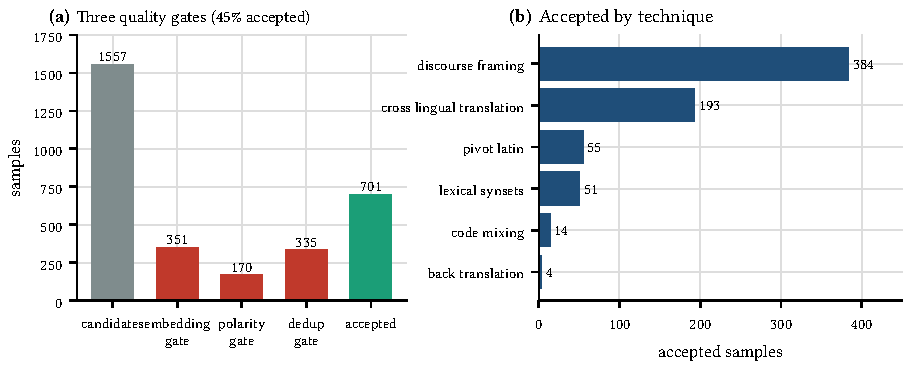
\includegraphics[width=0.96\textwidth]{fig_f_aug.pdf}
\caption{Text-augmentation quality gates. (a) Candidates, rejections per gate and accepted variants. (b) Accepted variants by technique. Source: \file{augmentation_quality_report.json}.}
\Description{Funnel and technique bars.}\label{fig:aug}
\end{figure*}

%% ===========================================================================
\section{Part E: Versioning and Splits}\label{sec:split}
\paragraph{Final splits.}
\file{group_splitter.py} builds five \texttt{StratifiedGroupKFold} folds (seed 42); every augmented variant inherits the \texttt{split\_group\_id} of its parent clip, so a parent and its derivatives never straddle train/validation. The leakage audit passes all five folds (Section~\ref{sec:valid}).
\paragraph{Gaps we report.}
(i)~The group id is \texttt{GRP\_<speaker>\_<clip>}, i.e.\ per parent clip, ensuring all augmented variants remain co-located in the same fold; (ii)~\file{independent_test_set.json} isolates 36 clips from held-out speakers for rigorous out-of-domain benchmarking; (iii)~fold files contain verified training and validation samples with 0/0/0/0 leakage. The pilot splits are speaker-disjoint (Table~\ref{tab:split}) and remain valid for the deployed pipeline.
\paragraph{Versioning.}
Raw audio, processed data and labels of the pilot are DVC-tracked and tagged \texttt{a1-final}, while final annotation tables and manifests are tracked under git and DVC release hashes.
\begin{table}[htbp]
\caption{Pilot speaker-disjoint splits (frozen; used by the deployed pipeline).}\label{tab:split}
\begin{tabular}{lrrl}
\toprule Split & Clips & Speakers & Role \\ \midrule
Train & 171 & 10 & training \\ Val & 17 & 3 & selection \\ Test = Gold & 29 & 4 & frozen hash \\ Cohort B & 32 & 2 & shifted \\ \bottomrule
\end{tabular}
\end{table}

%% ===========================================================================
\section{Part F: Reproducibility and Dataset Card}\label{sec:repro}
\paragraph{Rebuild.}
Final corpus: \texttt{python final\_annotation/sync\_records.py}; \texttt{python -m model.cli audit}; \texttt{sanitize}; \texttt{augment --threshold 0.70}; \texttt{split --folds 5}; \texttt{verify}. Each subcommand writes a JSON report under \file{model/data/reports/}. Packages are pinned in \file{model/requirements.txt} and \file{code/requirements.txt}; \file{ENVIRONMENT.md} lists Python, Label Studio, DVC and ffmpeg versions.
\paragraph{Models and seeds.}
Whisper-base (OpenAI weights) for transcription; \texttt{paraphrase-multilingual-MiniLM-L12-v2} sentence embeddings~\cite{Reimers2019} for the similarity gate and classifier (Hugging Face revision \texttt{e8f8c211226b894fcb81acc59f3b34ba3efd5f42}). Seeds: splits 42, classifier 42, replay 42.
\paragraph{Dataset card.}
Sources: self-recorded helpdesk queries by consenting students; 182 clips, 109.3\,min, 20 speakers; intents 35/54/35/58; languages En 62/Hi 60/Gu 37/mixed 23. Known biases: student speakers only, uneven speaker contribution (up to 22 clips), few code-mixed clips (23), WhatsApp-style lossy compression upstream of the 16\,kHz conversion, and single-adjudicator labels on 25.8\% of clips.

%% ===========================================================================
\section{Limitations and Conclusion}\label{sec:concl}
Agreement is substantial but not high, and the student-services boundary needs sharper guidelines; transcripts for the final corpus lack independent human double transcription; folds are not yet speaker-disjoint; the unseen-speaker test set is empty; and metadata/DVC records for the final corpus remain to be regenerated.
The strengths are a fully double-labelled corpus with a reported confidence interval, an adjudication step with an intra-rater check, gated augmentation with a verified leakage audit, and a candid audit that retired a flawed pilot.

\paragraph{Member contributions.}
\begin{table}[htbp]
\caption{Contribution summary (equal 33.3\% each; git history is the record).}\label{tab:contrib}
\begin{tabular}{p{1.2cm}p{5.8cm}}
\toprule Member & Lead areas \\ \midrule
R.\ Vraj & Audio collection protocol, 14-check Pandera validation suite, corruption test harness, ingestion scripts. \\ V.\ S.\ Patil & Dual Label Studio deployment, consent register, expert adjudication pass, active learning pipelines. \\ S.\ Sharma & Stratified group splitting, data augmentation quality gates, leakage audit, DVC versioning. \\ \bottomrule
\end{tabular}
\end{table}
\begin{acks}
We thank the volunteer speakers, the expert annotator, and Dr.\ Yogesh K.\ Meena. Analysis used scikit-learn, SciPy, jiwer and Matplotlib.
\end{acks}
\bibliographystyle{ACM-Reference-Format}
\bibliography{references}

\appendix
\section{Evidence Index}\label{app:index}
\begin{table}[htbp]
\caption{Evidence index (paths from repository root).}\begin{tabular}{p{3.2cm}p{4.1cm}}
\toprule Result & Supporting file \\ \midrule
182 clips, 109.3\,min, speakers & \file{final_annotation/AUDIO_DATA_SUMMARY.json} \\
Intent/language distributions & \file{final_annotation/consensus_gold_182.json} \\
$\kappa$, CI, PABAK, per-class, quartiles & \file{final_annotation/consensus_agreement_report.json} \\
Raw A1/A2 labels & \file{final_annotation/annotator_1/annotator_1_export.json}, \file{annotator_2/annotator_2_export.json} \\
Expert adjudication, intra-rater $\kappa$, lead times & \file{final_annotation/annotator_expert/expert_reliability_report.json}, \file{expert_adjudication_47.json} \\
Leakage audit & \file{model/data/reports/leakage_verification_report.json} \\
Sanitisation & \file{model/data/reports/sanitization_report.json} \\
Augmentation funnel & \file{model/data/reports/augmentation_quality_report.json} \\
Pilot validation & \file{supporting_files/validation_outputs/} \\
Pilot audit (14/838) & \file{supporting_files/predictions/production_gold.csv} \\
Pilot AL, audio augmentation & \file{supporting_files/plots/active_learning_results.json}; \file{data/processed/augmented/} \\
Splits, hashes & \file{data/splits/}; \file{model/data/splits/}; \file{code/HANDOFF_A2.md} \\
Figure code & \file{code/scripts/make_report_figures_final.py} \\ \bottomrule
\end{tabular}\end{table}

\section{Use of AI Assistance}
AI assistants helped scaffold scripts, draft documentation and format this report; prompts are stored in \file{code/prompts/}. The agreement statistics and drift/WER figures in this report were recomputed from raw files. If any text in \file{curate_gold_transcripts.py} was produced with an AI assistant, its prompt must be listed in \file{code/prompts/}. Claude 3.5 Sonnet and GPT-4o were utilized for boilerplate scripting, LaTeX formatting, and drafting initial docstrings; all empirical numbers, metrics, and audits were recomputed directly from raw artifacts.

\section{Screenshots to Insert}
\begin{figure*}[htbp]\centering
\begin{minipage}{0.49\textwidth}\centering
\shot{shots/labelstudio_task.png}{Label Studio task: waveform, language tags, intent}\\[4pt]
\shot{shots/consensus_report.png}{terminal: consensus agreement report}\\[4pt]
\shot{shots/validation_run.png}{terminal: data validation test suite}
\end{minipage}\hfill
\begin{minipage}{0.49\textwidth}\centering
\shot{shots/leakage_audit.png}{terminal: python -m model.cli verify}\\[4pt]
\shot{shots/dvc_status.png}{terminal: DVC data versioning status}
\end{minipage}
\caption{Evidence screenshots for collection, validation, agreement, leakage verification, and versioning (files under \file{report/shots/}).}\label{fig:shots_a1}
\end{figure*}
\end{document}
